% Chapter 1

\chapter{Introducción general} % Main chapter title

\label{Chapter1} % For referencing the chapter elsewhere, use \ref{Chapter1} 
\label{IntroGeneral}

En este capítulo se expone la necesidad que dio origen al desarrollo del trabajo. Se presenta el concepto de cultivo vertical y el estado del arte de su integración con la tecnología. Asimismo, se explican el objetivo y los alcances del trabajo.

%----------------------------------------------------------------------------------------

% Define some commands to keep the formatting separated from the content 
\newcommand{\keyword}[1]{\textbf{#1}}
\newcommand{\tabhead}[1]{\textbf{#1}}
\newcommand{\code}[1]{\texttt{#1}}
\newcommand{\file}[1]{\texttt{\bfseries#1}}
\newcommand{\option}[1]{\texttt{\itshape#1}}
\newcommand{\grados}{$^{\circ}$}

%----------------------------------------------------------------------------------------

%\section{Introducción}

%----------------------------------------------------------------------------------------
\section{Agricultura vertical como solución sostenible}

%\LaTeX{} no es \textsc{WYSIWYG} (What You See is What You Get), a diferencia de los procesadores de texto como Microsoft Word o Pages de Apple o incluso LibreOffice en el mundo open-source. En lugar de ello, un documento escrito para \LaTeX{} es en realidad un archivo de texto simple o llano que \emph{no contiene formato} . Nosotros le decimos a \LaTeX{} cómo deseamos que se aplique el formato en el documento final escribiendo comandos simples entre el texto, por ejemplo, si quiero usar texto en itálicas para dar énfasis, escribo \verb|\it{texto}| y pongo el texto que quiero en itálicas entre medio de las llaves. Esto significa que \LaTeX{} es un lenguaje del tipo \enquote{mark-up}, muy parecido a HTML.

Con una población mundial que supera los 8000 millones de personas y continúa en crecimiento \cite{PEOPLE}, la agricultura enfrenta el desafío de volverse más eficiente y sostenible \cite{AGUA} \cite{FAO} \cite{SANTANDER}. En este contexto, los cultivos verticales emergen como una solución innovadora que optimiza el uso del espacio y los recursos, especialmente en entornos urbanos, donde el suelo es limitado y costoso.

Este tipo de agricultura utiliza técnicas como la hidroponía, que permite un uso preciso del agua, y la aeroponía, que maximiza el oxígeno disponible para las raíces. Además, las granjas verticales aprovechan áreas infrautilizadas, como edificios abandonados o naves industriales, y permiten cultivar alimentos en zonas donde la agricultura tradicional resulta dificil de desarrollar. Así, se logra una mayor densidad de cultivo y se contribuye a la sostenibilidad al reducir el uso de pesticidas y fertilizantes.

Aunque los cultivos verticales requieren un alto nivel de tecnología y tienen costes energéticos asociados, su capacidad para ahorrar recursos, disminuir la huella de carbono y fomentar la producción de alimentos en espacios reducidos y con menor dependencia de factores climáticos, justifica la inversión en su desarrollo y expansión \cite{alhwarin2020vertical}.

Este método, también conocido como agricultura urbana, permite el crecimiento de plantas en interiores sin necesidad de luz solar directa, gracias a la aplicación de tecnologías agrícolas avanzadas. Estas optimizan las condiciones de cultivo, lo que facilita la propagación de plantas jóvenes y la producción de alimentos más saludables sin el uso de pesticidas.

Además, maximizan la producción al emplear sistemas de iluminación especializados de nueva generación, diseñados para estructuras multicapa. Gracias a esta tecnología, es posible obtener mayores rendimientos en un espacio reducido, consolidando a la agricultura vertical como una solución sostenible y eficiente para la producción de alimentos en entornos urbanos y con recursos limitados \cite{SANTANDER}.

\subsection{Tipos de cultivos verticales}

%https://agroquivir.com/agricultura-vertical-como-funciona-y-tipos/

%Si sos nuevo en \LaTeX{}, hay un muy buen libro electrónico - disponible gratuitamente en Internet como un archivo PDF - llamado, \enquote{A (not so short) Introduction to \LaTeX{}}. El título del libro es generalmente acortado a simplemente \emph{lshort}. Puede descargar la versión más reciente en inglés (ya que se actualiza de vez en cuando) desde aquí:
%\url{http://www.ctan.org/tex-archive/info/lshort/english/lshort.pdf}

%Se puede encontrar la versión en español en la lista en esta página: \url{http://www.ctan.org/tex-archive/info/lshort/}

Existen distintos tipos de agricultura vertical, que optimizan el crecimiento de las plantas sin grandes extensiones de suelo y emplean estructuras especializadas para maximizar la producción.
A continuación, se describen los principales tipos de cultivos verticales y sus características.

\subsubsection{Hidroponía}
La hidroponía es un método de cultivo sin suelo que suministra nutrientes a las plantas a través de una solución acuosa, con raíces en un medio inerte como lana de roca o perlita. Es un sistema eficiente en el uso de agua, permite un control preciso de nutrientes y favorece una mayor densidad de cultivo y un crecimiento más rápido que los métodos tradicionales \cite{SANTANDER} \cite{CULTIVOS:TIPOS}.
\subsubsection{Aeroponía}
La aeroponía es un método de cultivo en el que las raíces de las plantas quedan suspendidas en el aire y se rocían con una solución nutritiva. Maximiza la oxigenación, acelera el crecimiento y optimiza el uso de nutrientes, aunque requiere un control preciso para evitar la desecación de las raíces \cite{SANTANDER} \cite{CULTIVOS:TIPOS}.
\subsubsection{Acuaponía}
La acuaponía combina la cría de peces con la hidroponía, utilizando los desechos de los peces como fertilizante para las plantas, mientras estas purifican el agua. Es un sistema sostenible que minimiza el desperdicio, promueve la biodiversidad y es viable en entornos urbanos y rurales \cite{CULTIVOS:TIPOS}.

%Acá tiene un ejemplo de una ``subsubsección'' que es el cuarto nivel de ordenamiento del texto, después de capítulo, sección y subsección.  Como se puede ver, las subsubsecciones no van numeradas en el cuerpo del documento ni en el índice.  El formato está definido por la plantilla y no debe ser modificado.

\subsection{Sistemas de agricultura vertical más conocidos}
Los sistemas de agricultura vertical varían según el tipo de cultivo y la técnica más adecuada para cada necesidad.
A continuación, se describen los principales sistemas de cultivos verticales y sus características.

\subsubsection{Sistemas de torre}
Las torres verticales permiten el cultivo de plantas en estructuras cilíndricas apiladas, con el fin de maximizar el uso del espacio y facilitar tanto la recolección como el mantenimiento. Este sistema es ideal para cultivos de hoja verde y hierbas, y se integra fácilmente en espacios urbanos como balcones y terrazas \cite{CULTIVOS:TIPOS}.

\subsubsection{Sistemas en rack o estanterías}
Estos sistemas emplean estanterías apiladas donde las plantas crecen en bandejas o contenedores, son ideales para invernaderos y ambientes controlados. Facilitan el riego, la recolección y el monitoreo, al mismo tiempo que se optimiza el uso del espacio.
Los sistemas en rack o estanterías son especialmente útiles para cultivos que requieren diferentes niveles de luz y humedad \cite{CULTIVOS:TIPOS}.

\subsubsection{Sistemas montados en pared}
En estos sistemas, las plantas crecen en módulos montados en paredes. Su integración en la arquitectura no solo optimiza el espacio, sino que también aporta beneficios estéticos y funcionales.
Los jardines verticales pueden mejorar la calidad del aire y contribuir al aislamiento térmico de los edificios \cite{CULTIVOS:TIPOS}.

\subsubsection{Sistemas de bastidor en A}
El bastidor en forma de ``A`` proporciona una estructura estable y accesible para el cultivo vertical, lo que a su vez facilita el acceso a la luz y el riego.
Este diseño es particularmente útil para cultivos que necesitan un soporte adicional, como tomates y pepinos, y puede ser utilizado tanto en interiores como en exteriores \cite{CULTIVOS:TIPOS}.

\subsubsection{Sistemas de contenedores}
Estos sistemas utilizan contenedores apilables que pueden moverse y configurarse según las necesidades, adaptándose a diversos entornos y tipos de cultivo.
Los contenedores son ideales para cultivos modulares y pueden ser personalizados para optimizar el uso del espacio y los recursos \cite{CULTIVOS:TIPOS}.
%Si estás escribiendo un documento con mucho contenido matemático, entonces es posible que desees leer el documento de la AMS (American Mathematical Society) llamado, \enquote{A Short Math Guide for \LaTeX{}}. Se puede encontrar en línea en el siguiente link: \url{http://www.ams.org/tex/amslatex.html} en la sección \enquote{Additional Documentation} hacia la parte inferior de la página.


%----------------------------------------------------------------------------------------

\section{Motivación}

Este trabajo surge como un desarrollo de interés personal, impulsado por el deseo de contribuir positivamente al desarrollo sustentable y la optimización de los recursos naturales en la producción de alimentos. En la actualidad, el crecimiento de la población mundial y el aumento en la demanda de productos agrícolas presentan grandes desafíos ambientales y económicos.

La producción tradicional de alimentos enfrenta dificultades debido a la explotación intensiva de suelos, el uso excesivo de fertilizantes y pesticidas y el desperdicio de recursos esenciales como el agua. Con el fin de maximizar sus ganancias, muchas empresas recurren a métodos poco sostenibles que generan un impacto ambiental negativo, y afectan la biodiversidad, la calidad del suelo y el bienestar de las comunidades locales que dependen de estas fuentes de producción.

Uno de los problemas más críticos en la agricultura tradicional es el significativo desperdicio de agua en el riego. Se estima que se desperdicia hasta el 84 \% del agua utilizada para riego \cite{CLARIN}. Esta pérdida ocurre principalmente por evaporación, drenaje o absorción ineficiente. En un contexto donde la crisis hídrica es una amenaza global, desarrollar sistemas más sostenibles se vuelve una necesidad urgente.

Por otro lado, existe una creciente preocupación entre los consumidores sobre la calidad y procedencia de los alimentos. Cada vez más personas optan por un estilo de vida saludable, adoptando hábitos de consumo responsables, como el vegetarianismo, el veganismo y el autocultivo. Sin embargo, muchos de estos consumidores no cuentan con espacios adecuados ni conocimientos técnicos para producir sus propios alimentos, lo que genera una gran oportunidad para soluciones tecnológicas que faciliten la agricultura doméstica.

A partir de estas problemáticas, nació la motivación para desarrollar un sistema hidropónico inteligente, que no solo optimice el uso del agua, sino que también permita una gestión eficiente del cultivo con mínima intervención del usuario. Este trabajo ofrece una alternativa viable y escalable para la producción de alimentos frescos, reduce la dependencia de sistemas agrícolas tradicionales y promueve un modelo más sustentable para el futuro.


\section{Estado del arte}
Durante la etapa de investigación, se llevó a cabo una búsqueda de productos comerciales tanto en el mercado local como en el internacional. Se identificaron diversas soluciones con características similares al sistema desarrollado.

A continuación, se describen los productos identificados.

\subsubsection{NIDO PRO}
El NIDO PRO, figura \ref{fig:nido_pro}, es un sistema hidropónico inteligente para cultivos verticales que permite controlar la solución nutritiva a través de una aplicación móvil. Facilita la gestión del pH y la conductividad eléctrica (CE), con algoritmos que realizan comprobaciones diarias para garantizar la estabilidad de la solución nutritiva. Además, admite hasta cuatro ranuras para fertilizantes líquidos y ajustes de pH, lo que optimiza el proceso de nutrición de las plantas \cite{NIDO:PRO}.

\begin{figure}[H]
	\centering
	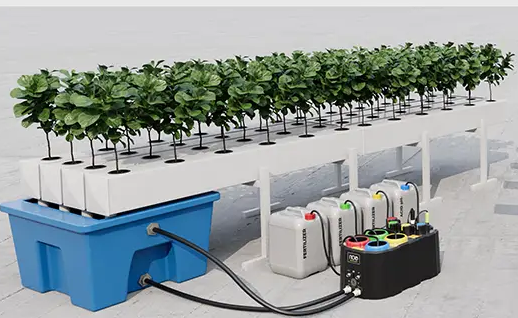
\includegraphics[scale=.55]{./Figures/nido:pro.png}
	\caption{Ilustración del módulo NIDO PRO conectado a un sistema hidropónico horizontal\protect\footnotemark.}
	\label{fig:nido_pro}
\end{figure}


\footnotetext{Imagen tomada de \href{https://www.agrointec.com/producto/nidopro-sistema-hidroponico-inteligente-cultivo-vertical/}
{https://acortar.link/uEmExI}}


%https://www.agrointec.com/producto/nidopro-sistema-hidroponico-inteligente-cultivo-vertical/?utm_source=chatgpt.com

\subsubsection{Xiaomi Mi Flower Care Plant Sensor}
El Xiaomi Mi Flower Care Plant Sensor, figura \ref{fig:xiaomi}, monitorea variables ambientales como luz, humedad, nutrientes y temperatura del sustrato. Los sensores se conectan a aplicaciones móviles, lo que permite realizar un seguimiento detallado y controlar las condiciones del cultivo de manera precisa \cite{XIAOMI}.

\begin{figure}[H]
	\centering
	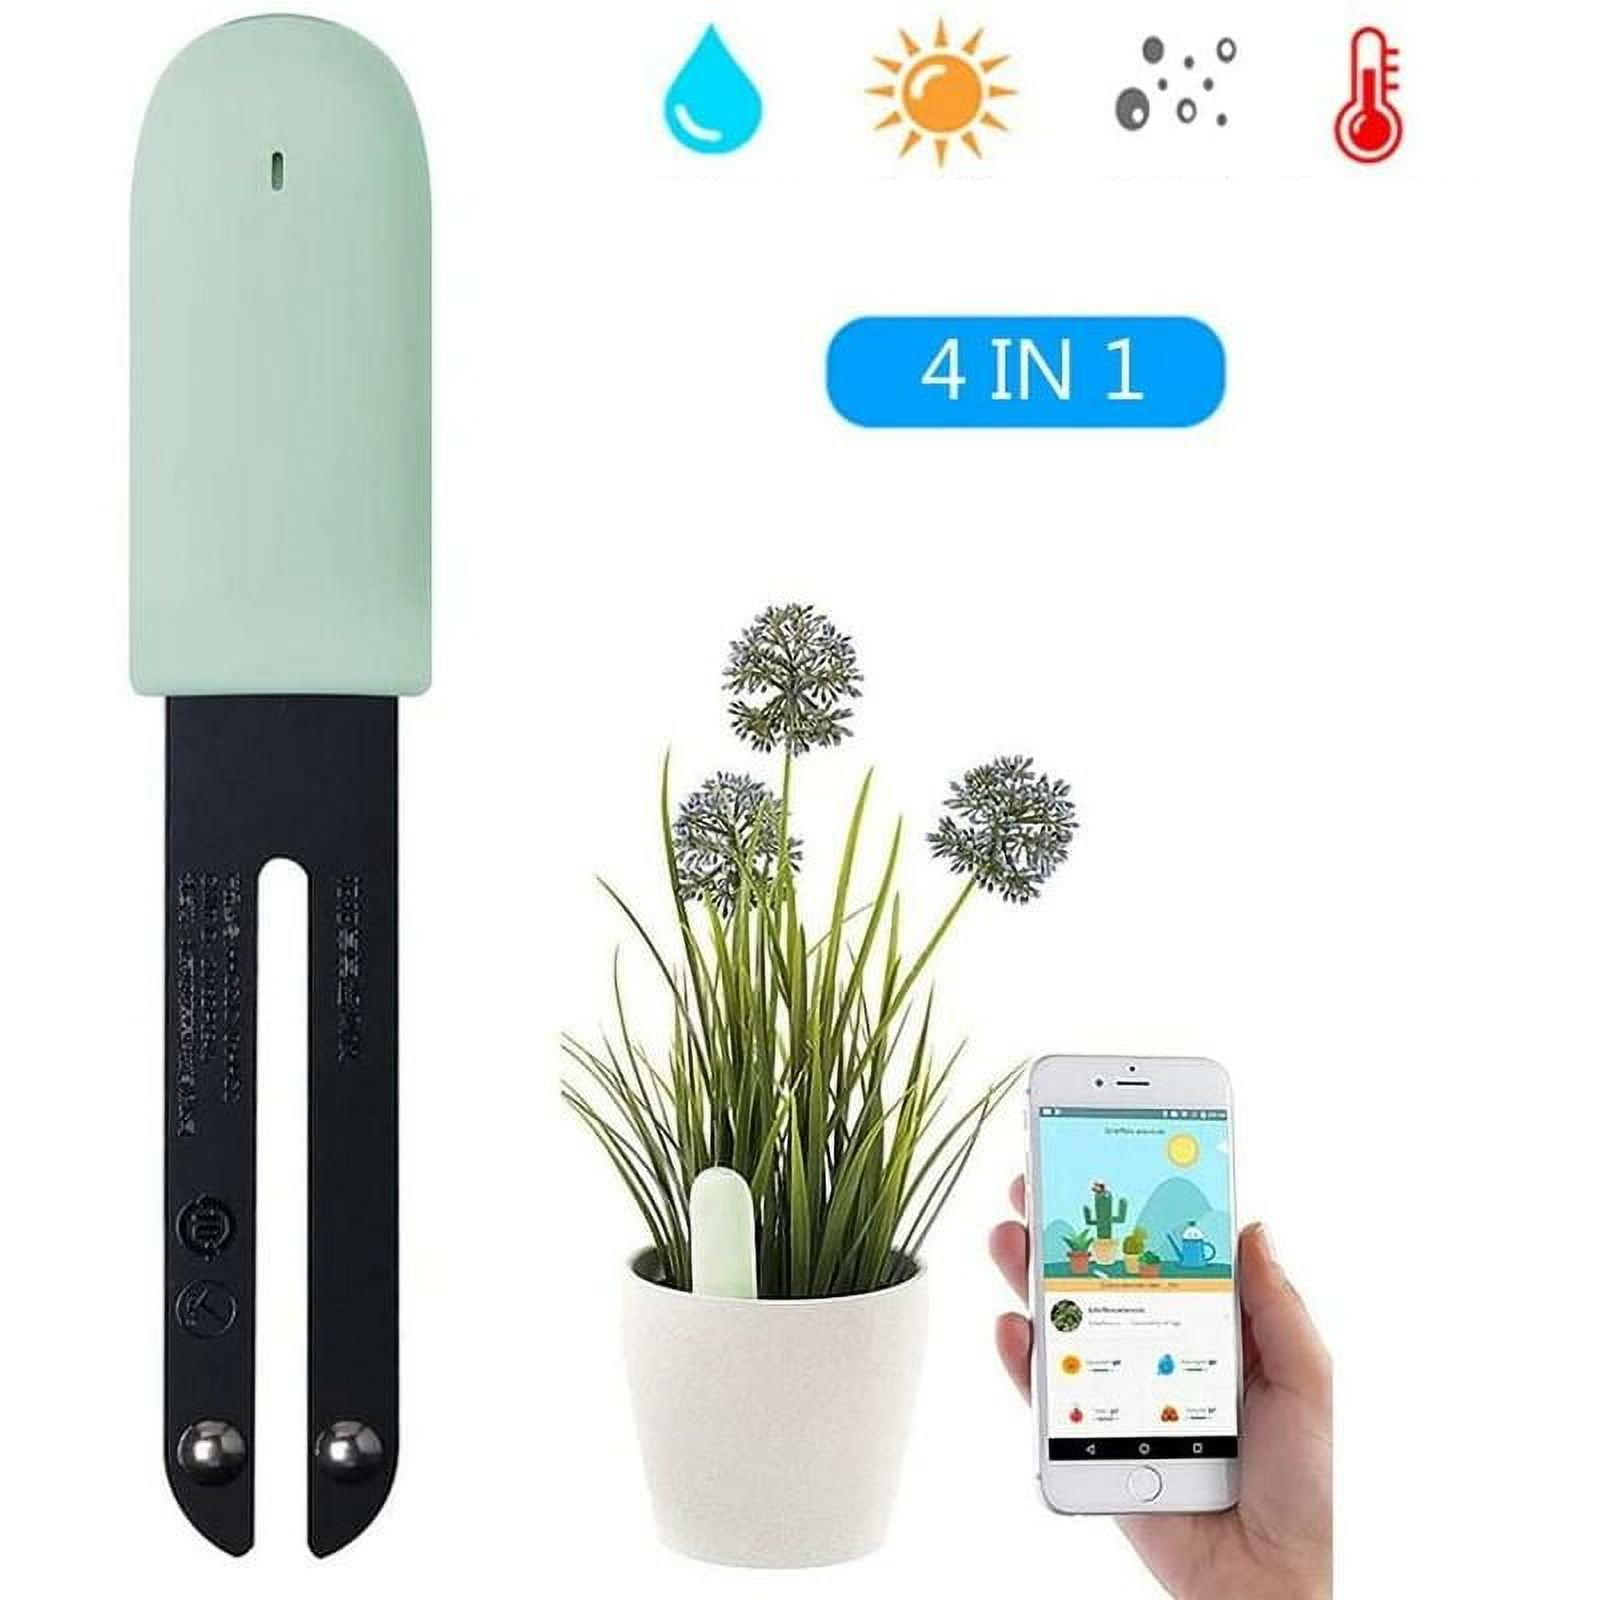
\includegraphics[scale=.14]{./Figures/xiaomi.jpg}
	\caption{Ilustración del dispositivo Xiaomi Mi Flower Care Plant Sensor y sus prestaciones\protect\footnotemark.}
	\label{fig:xiaomi}
\end{figure}


\footnotetext{Imagen tomada de \href{https://www.walmart.com/ip/Xiaomi-Flower-Care-Soil-Tester-Intelligent-Plant-Monitor-Bluetooth-4-1-Soil-Tester-Automatically-Monitors-Humidity-Light-Fertility-Temperature-Levels/15639619580}
{https://acortar.link/bVNwHC}}



%https://elpais.com/tecnologia/tu-tecnologia/2024-12-07/dispositivos-tecnologicos-para-que-tus-plantas-sean-la-envidia-de-cualquiera.html?utm_source=chatgpt.com

\subsubsection{Kit de Riego Hydro de Konyks}
El sistema de riego inteligente Konyks, figura \ref{fig:kit_konyks}, permite controlar la llave de paso de forma remota mediante una aplicación móvil y asistentes de voz como Alexa, Google Home o Siri. Incorpora un medidor de caudal para monitorear el consumo de agua y una toma con relé RF que amplía la conectividad hasta 60 m y permite gestionar hasta cuatro grifos. Además, ofrece automatización programable según el clima y los horarios, lo que optimiza el uso del agua y facilita la gestión del riego desde cualquier lugar \cite{KONIX}.

\begin{figure}[H]
	\centering
	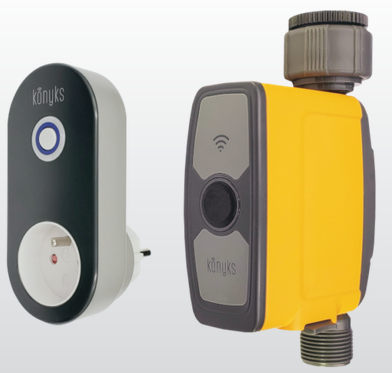
\includegraphics[scale=.4]{./Figures/kit_konyks.png}
	\caption{Sistema de riego conectado Konyks\protect\footnotemark.}
	\label{fig:kit_konyks}
\end{figure}

\footnotetext{Imagen tomada de \url{https://konyks.com/es/producto/hydro-kit/}}




%https://elpais.com/tecnologia/tu-tecnologia/2024-12-07/dispositivos-tecnologicos-para-que-tus-plantas-sean-la-envidia-de-cualquiera.html?utm_source=chatgpt.com

\subsubsection{Smart 9 Pro de Click \& Grow}
El Smart Garden 9 PRO, figura \ref{fig:smart_garden}, es un sistema de cultivo doméstico automatizado con control a través de una aplicación. Ofrece riego automático, iluminación ajustable tanto por control táctil como desde la app, y un suministro equilibrado de nutrientes y oxígeno en las raíces. Permite cultivar hierbas, frutas, ensaladas y flores durante todo el año, con la opción de utilizar cápsulas presembradas (más de 50 variedades disponibles) o semillas propias. Incluye un set inicial con cápsulas de tomate, albahaca y lechuga \cite{SMART:9}.

\begin{figure}[H]
	\centering
	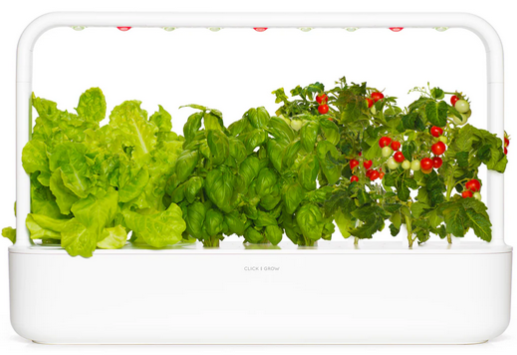
\includegraphics[scale=.6]{./Figures/smart_garden.png}
	\caption{Módulo Smart Garden 9 PRO\protect\footnotemark.}
	\label{fig:smart_garden}
\end{figure}

\footnotetext{Imagen tomada de \url{https://www.clickandgrow.com/products/the-smart-garden-9-pro}}

%https://elpais.com/tecnologia/tu-tecnologia/2024-12-07/dispositivos-tecnologicos-para-que-tus-plantas-sean-la-envidia-de-cualquiera.html?utm_source=chatgpt.com

\section{Objetivos y alcances}

A continuación, se presentan los objetivos del trabajo.

\subsection{Objetivos}
\begin{itemize}
    \item Desarrollar un prototipo de sistema hidropónico automatizado para monitoreo y gestión eficiente del cultivo.
    \item Implementar la conexión de sensores para medir temperatura, humedad, pH, conductividad eléctrica, nivel de agua e intensidad lumínica.
    \item Diseñar una interfaz web y móvil que permita la supervisión y configuración remota del sistema.
    \item Evaluar el rendimiento del sistema en comparación con métodos tradicionales, midiendo eficiencia y productividad.
    \item Poner en práctica los conocimientos adquiridos a lo largo de la carrera de especialización en sistemas embebidos.
\end{itemize}

\subsection{Alcances}

A continuación, se presentan los alcances del trabajo.

\begin{itemize}
    \item El sistema permite el monitoreo en tiempo real y la gestión automatizada del riego, iluminación y ventilación.
    \item El dispositivo se enfocó en cultivos hidropónicos verticales de pequeña y mediana escala.
    \item Se realizaron pruebas de funcionamiento y validación en un entorno controlado, pero no se contempló una implementación comercial en esta etapa.
\end{itemize}

%Si estás familiarizado con \LaTeX{}, entonces podés explorar la estructura de directorios de esta plantilla y proceder a personalizarla agregando tu información en el bloque \emph{INFORMACIÓN DE LA PORTADA} en el archivo \file{memoria.tex}.  

%Se puede continuar luego modificando el resto de los archivos siguiendo los lineamientos que se describen en la sección \ref{sec:FillingFile} en la página \pageref{sec:FillingFile}.

%Debés asegurarte de leer el capítulo \ref{Chapter2} acerca de las convenciones utilizadas para las Memoria de los Trabajos Finales de la \degreename.

%Si sos nuevo en \LaTeX{}, se recomienda que continúes leyendo el documento ya que contiene información básica para aprovechar el potencial de esta herramienta.


%----------------------------------------------------------------------------------------